\documentclass[tikz,crop]{standalone}

\usepackage[T1]{fontenc}
\usepackage{multirow, makecell}
\usepackage[tt=false,type1=true]{libertine}
%%% \usepackage[varqu]{zi4}
%%% \usepackage{newtxmath}
\usepackage{listings}
\usepackage[dvipsnames]{xcolor}
\usepackage{tikz}
%%% \usepackage{bbding}
\usetikzlibrary{arrows,backgrounds,external,fit,positioning,shadows,shapes,shapes.arrows,shapes.multipart}
% \tikzexternalize

% COLORS: https://colorkit.co/palette/c7522a-e5c185-fbf2c4-74a892-008585/
\definecolor{palet1}{HTML}{c7522a}
\definecolor{palet2}{HTML}{e5c185}
\definecolor{palet3}{HTML}{fbf2c4}
\definecolor{palet4}{HTML}{74a892}
\definecolor{palet5}{HTML}{008585}

\lstset{
    % backgroundcolor=\color{backcolour},
    % stringstyle=\color{codepurple},
    % commentstyle=\color{codegreen},
    keywordstyle=\bfseries\color{magenta},
    numberstyle=\tiny\color{codegray},
    basicstyle=\ttfamily\tiny,
    % captionpos=b,
    escapeinside={/@}{@/},
    % breakatwhitespace=false,
    % breaklines=true,
    % keepspaces=true,
    % numbers=left,
    % numbersep=5pt,
    % showspaces=false,
    % showstringspaces=false,
    % showtabs=false,
    % tabsize=2
}

% \colorlet{ml-model-bg}{CornflowerBlue!10}

\begin{document}
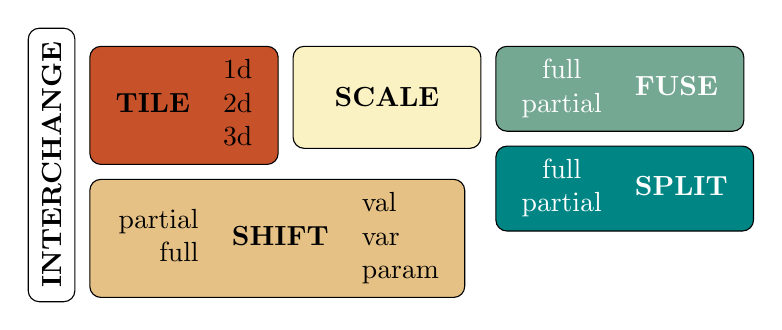
\begin{tikzpicture}[
  t/.style={draw, rounded corners}
  ]
  \node[t,fill=palet2] (shift) {
    \begin{tabular}{rcl}
      \multirow{3}{3em}{\makecell[r]{partial\\full}}& \multirow{3}*{\textbf{SHIFT}} & val \\
      & & var \\
      & & param
    \end{tabular}
  };
  \node[t,fill=palet1,anchor=south west, yshift=0.5em] (tile) at (shift.north west) {
    \begin{tabular}{cl}
      \multirow{3}*{\textbf{TILE}} & 1d \\
      & 2d \\
      & 3d
    \end{tabular}
  };
  \node[t,fill=palet3, inner sep=15,anchor=north west, xshift=0.5em] (scale) at (tile.north east) {
    \textbf{SCALE}
  };
  \node[t,fill=palet4,text=white, anchor=north west, xshift=0.5em] (fuse) at (scale.north east) {
    \begin{tabular}{cl}
      full & \multirow{2}*{\textbf{FUSE}} \\
      partial &
    \end{tabular}
  };
  \node[t,fill=palet5,text=white, anchor=north west, yshift=-0.5em] (split) at (fuse.south west) {
    \begin{tabular}{cl}
      full & \multirow{2}*{\textbf{SPLIT}} \\
      partial &
    \end{tabular}
  };
  \node[t,fill=white,rotate=90, inner sep=0.5em, anchor=south, yshift=0.5em] (interchange) at (tile.south west) {
    \textbf{INTERCHANGE}
  };

  \begin{scope}[on background layer]
    % \path node[rounded corners, fill=blue, fit=(shiftpf) (shift) (shiftvvp)] {};
    % \path node[rounded corners, fill=red, fit=(tile) (tileds)] {};
  \end{scope}
\end{tikzpicture}
\end{document}
